\vspace*{1em}

The following result can be used to conclude if an algebraic number is irrational.
\vspace*{0.5em}
\begin{theorem}[Rational Root Theorem]
Let $a/b$ be a rational number in reduced form such that it's a root of a polynomial
\[P(T) = c_dT^d + c_{d-1}T^{d-1} + \cdots + c_1T + c_0\]
where $c_i \in \zz$. Then $a\mid c_0$ and $b\mid c_d$.
\end{theorem}
\begin{proof}
By assumption
\[P\left(\frac{a}{b}\right) = c_d\left(\frac{a}{b}\right)^d + c_{d-1}\left(\frac{a}{b}\right)^{d-1} + \cdots + c_1\left(\frac{a}{b}\right) + c_0 = 0\]
Then
\[c_da^d + c_{d-1}a^{d-1}b + \cdots c_1ab^{d-1} + c_0b^d = 0\]
Therefore,
\begin{align*}
c_da^d &= -b(c_{d-1}a^{d-1}+\cdots + c_1ab^{d-2})\text{; and}\\[0.5em]
c_0b^d &= -a(c_da^{d-1} +\cdots + c_1b^{d-1})
\end{align*}
Therefore $b\mid c_da^d$ and $a\mid c_0b^d$. Since $\gcd(a,b) = 1$, hence $\gcd(a,b^d) = \gcd(a^d,b) = 1$. Thus $b\mid c_d$ and $a\mid c_0$, by Lemme \ref{primediv}.
\end{proof}

\emph{e.g.}\quad For $\alpha = 2\sqrt{2} + \sqrt{3}$, we found $P(T) = T^4 - 22T^2 + 25$ is such that $P(\alpha) = 0$. Suppose $\alpha = a/b$ is rational, then $a\mid 25$ and $b\mid 1$. Therefore $a/b \in \set{\pm 1, \pm 5, \pm 25}$ but none of them equal $2\sqrt{2} + \sqrt{3}$.

\vspace*{1em}

\begin{example}[in-class]
$\sqrt{3} + \sqrt{5}$ is algebraic and irrational.
\end{example}

\vspace*{1em}

{\bf Examples of transcendental number.} Note that $\cc$ is uncountable but the set of all algebraic numbers is countable. Therefore there are uncountably many transcendental numbers.

\vspace*{1em}

\begin{theorem}[Lindemann \& Weierstrass, 1800's]
$\pi$ and $e$ are transcendental.\\
\\
\textnormal{(But we don't yet know if $e + \pi$ is transcendental, for example.)}
\end{theorem}

\vspace*{1em}

\begin{corollary}[ancient]
We cannot square the circle. That is, using only a straight ruler and compass we cannot construct a square whose area is equal to $\pi$.
\end{corollary}

\vspace*{1.5em}

{\bf Other suspects.} Let $k \geq 1$ be an integer, then
\[\zeta_k = 1 + \frac{1}{2^k} + \frac{1}{3^k} + \frac{1}{4^k} + \cdots\]
converges when $k>1$.
\begin{proof}[{\bf Facts}]\renewcommand{\qedsymbol}{}
\begin{itemize}
\item[(1)] $\displaystyle \zeta_2 = \sum_{n=1}^\infty\frac{1}{n^2} = \frac{\pi^2}{6}$ (Basel problem, solved by Euler in 1734). $\zeta_2$ is transcendental.\\[0.5em]
\hspace*{2.8em} More generally, $\zeta_{2r} = \pi^{2r}\cdot\text{(rational number)}$; $\zeta_{2r}$ transcendental.
\end{itemize}
\begin{itemize}[leftmargin=5.5em]
\item[(2)] $\displaystyle \zeta_3 = \sum_{n=1}^\infty\frac{1}{n^3}$ is irrational (Ap\'ery, 1979). We don't yet know if it is transcendental.
\item[(3)] Euler-Mascheroni constant $\displaystyle \gamma = \lim_{n\to \infty}\left(1 + \frac{1}{2} + \frac{1}{3} + \frac{1}{4} + \cdots + \frac{1}{n} - \ln(n+1)\right)$.\\[0.5em]
Open: is $\gamma$ rational?
\end{itemize}
\end{proof}

%\vspace*{1em}

{\bf\large Diophantine Approximation.} Recall that $\qq$ is \emph{dense} in $\rr$, i.e., for any $x \in \rr$ and $\epsilon > 0$, we can find a $q \in \qq$ such that $|x - q| < \epsilon$.

\vspace*{1em}

\begin{proposition}
Let $\alpha$ be any real number and $b$ a positive integer. Then there exists an integer $a$ such that 
\[\abs{x - \frac{a}{b}} \leq \frac{1}{2b}\]
\end{proposition}
\begin{proof}
Plot $\dfrac{1}{b}\zz$
\[\begin{tikzpicture}
    \draw[<->,thick] (-7,0)--(7,0);
	\foreach \x in {-6,-5,-4,-3,-2,-1,0,1,2,3,4,5,6}
    {
    \fill (\x,0) circle (1.5pt);
    }
    \node[] at (0,-0.55) {$\dfrac{0}{b}$};
    \node[] at (1,-0.55) {$\dfrac{1}{b}$};
    \node[] at (2,-0.55) {$\dfrac{2}{b}$};
    \node[] at (3,-0.55) {$\dfrac{3}{b}$};
    \node[] at (4,-0.55) {$\dfrac{4}{b}$};
    \node[] at (5,-0.55) {$\dfrac{5}{b}$};
    \node[] at (6,-0.55) {$\dfrac{6}{b}$};
    \node[] at (-1.15,-0.55) {$-\dfrac{1}{b}$};
    \node[] at (-2.15,-0.55) {$-\dfrac{2}{b}$};
    \node[] at (-3.15,-0.55) {$-\dfrac{3}{b}$};
    \node[] at (-4.15,-0.55) {$-\dfrac{4}{b}$};
    \node[] at (-5.15,-0.55) {$-\dfrac{5}{b}$};
    \node[] at (-6.15,-0.55) {$-\dfrac{6}{b}$};
\end{tikzpicture}\]
Then, say
\[\begin{tikzpicture}
    \draw[<->,thick] (-2.75,0)--(2.75,0);
	\foreach \x in {-2,2}
    {
    \fill (\x,0) circle (1.5pt);
    }
    \node[] at (2,-0.55) {$\dfrac{c+1}{b}$};
    \node[] at (-2.15,-0.55) {$-\dfrac{c}{b}$};
    \node[color=blue] at (0.5,-0.35) {$x$};
    \fill[color=blue] (0.5,0) circle (1.5pt);
\end{tikzpicture}\]
Between $c/b$ and $(c+1)/b$, choose the one closest to $x$ and define $a/b$ as such. So, 
\[\abs{x - \frac{a}{b}} \leq \frac{1}{2}\left(\text{length of $\left[\frac{a}{b},\frac{a+1}{b}\right]$}\right) = \frac{1}{2b}\]
\end{proof}
\vspace*{1em}
Sometimes, we have a far better deal\\[0.2em]
\emph{e.g.}\quad $\pi = 3.1415926$
\begin{itemize}
\item $a/b = 3.14 = 314/100 = 157/100$; $|\pi - a/b| \approx 0.00159$. Compared to $1/2b = 1/100 = 0.01$, it's $\sim 16\%$ off.
\item $a/b = 22/7 = 3.\overline{142857}$; $|\pi - a/b| \approx 0.0013$. Compared to $1/2b = 1/14 = 0.07$, it's only $\sim 2\%$ off.
\end{itemize}

Why do we care about this? To prove transcendence of numbers. For example, if we want to prove $\pi$ or $e$ is transcendental, then we have to show that for \emph{every} polynomial $P$ with integer coefficients, we must have $P(\pi),P(e) \neq 0$. That's a tall order, since there are infinitely such polynomials.\\
\\
One idea in transcendence theory, a rule of thumb, is that if you can approximate an irrational number $\alpha$ by rational (or algebraic) numbers very well, then $\alpha$ is likely to be transcendental.\\
\\
\emph{e.g.}\quad $e^x = 1 + x + \dfrac{x^2}{2!} + \dfrac{x^3}{3!} + \dfrac{x^4}{4!} + \cdots$. So,\\[-0.5em]
\[e = x + \dfrac{1}{2!} + \dfrac{1}{3!} + \dfrac{1}{4!} + \cdots\]
Terms in the series decrease very rapidly, since $n!$ increases rapidly as $n\to \infty$.
\vspace*{2em}

\begin{definition}
Let $a/b$ and $c/d$ be (reduced) fractions. The \emph{mediant} of $a/b$ and $c/d$ is
\[\dfrac{a}{b} \vee \dfrac{c}{d} \coloneqq \dfrac{a+c}{b+d}\]
\emph{e.g.}\quad $\dfrac{5}{3} \vee \dfrac{11}{17} = \dfrac{5+11}{3 + 17} = \dfrac{16}{20}$.
\end{definition}

\vspace*{1em}

\begin{proposition}
Let $a/b$ and $c/d$ be reduced fractions, then $a/b \vee c/d$ lies between $a/b$ and $c/d$.
\end{proposition}
\begin{proof}
Plot $(b,a)$ and $(d,c)$ in the Cartesian plane, say we get
\[\begin{tikzpicture}
    \draw[<->,thick] (-3,0)--(3,0);
	\draw[<->,thick] (0,-1.5)--(0,3);
	\draw[-,thick,color=indigo] (0,0)--(1,1);
	\draw[-,thick,color=purple] (0,0)--(-2,1.5);
	\draw[-,thick,color=teal] (0,0)--(-1,2.5);
	\draw[-,thick,color=teal] (0,0)--(-1,2.5);
	\draw[-,dashed] (-2,1.5)--(-1,2.5);	
	\draw[-,dashed] (1,1)--(-1,2.5);	
	\fill (-2,1.5) circle (1.5pt);
    \fill (1,1) circle (1.5pt);
    \fill (-1,2.5) circle (1.5pt);
    \node[] at (1.5,1.25) {\footnotesize $(b,a)$};
    \node[] at (-2.5,1.75) {\footnotesize $(d,c)$};
    \node[] at (-1.25,2.75) {\footnotesize $(b+d,a+c)$};
    \node[color=teal] at (-1,1.75) {\footnotesize $\ell_3$};
    \node[color=purple] at (-1.5,0.75) {\footnotesize $\ell_2$};
    \node[color=indigo] at (0.75,0.35) {\footnotesize $\ell_1$};
\end{tikzpicture}\]
Then note that
\begin{align*}
\frac{a}{b} &\text{ is the slope of {\color{indigo} $\ell_1$}}\\[0.5em]
\frac{c}{d} &\text{ is the slope of {\color{purple} $\ell_2$}}\\[0.5em]
\frac{a+c}{b+d} &\text{ is the slope of {\color{teal} $\ell_3$}}
\end{align*}
Therefore, as a rational number, $\dfrac{a}{b}\vee \dfrac{c}{d} = \dfrac{a+c}{b+d}$ lies between $\dfrac{a}{b}$ and $\dfrac{c}{d}$.
\end{proof}

\vspace*{1em}

\begin{definition}
Let $a/b$ be a reduced fraction; in particular $b>0$. The \emph{Ford circle atop $a/b$} is the circle of diameter $1/b^2$ that is above and tangent to the real line at the rational number $a/b$.
\[\begin{tikzpicture}[scale=2]
    \draw[thick,color=firebrick](-2,0.5) circle (0.5);
    \draw[thick,color=firebrick](-1,0.5) circle (0.5);
    \draw[thick,color=indigo](-1.5,0.125) circle (0.125);
    \draw[thick,color=firebrick](2,0.5) circle (0.5);
    \draw[thick,color=indigo](2.5,0.125) circle (0.125);
    \draw[<->,thick] (-3,0)--(3,0);
    \foreach \x in {-2,-1,0,1,2,2.5,-1.5}
    {
    \fill (\x,0) circle (1pt);
    }
    \node[] at (0,-0.2) {$0$};
    \node[] at (1,-0.2) {$1$};
    \node[] at (2,-0.2) {$2$};
    \node[] at (-1,-0.2) {$-1$};
    \node[] at (-2,-0.2) {$-2$};
    \node[] at (-1.5,-0.2) {\small $-3/2$};
    \node[] at (2.5,-0.2) {\small $5/2$};
    \node[draw,color=firebrick,thick](A) at (0.5,1.25) {\footnotesize diameter $=\dfrac{1}{1^2}$};
    \node[draw,color=indigo,thick](B) at (4,0.5) {\footnotesize diameter $=\dfrac{1}{2^2}$};
    \draw[dashed,color=firebrick,thick] (-0.5,0.5)--(A);
    \draw[dashed,color=indigo,thick] (2.625,0.125)--(B);
\end{tikzpicture}\]
Note that some Ford circles are tangent to each other.
\end{definition}

\vspace*{0.5in}

\subsection{Problems}
\vspace{0.1in}

\begin{problem}\label{Problem 6.1}\hfill
\begin{itemize}
\item[(a)] Find a nonzero rational polynomial $P(T)$ that has $\sqrt{5} + \sqrt[3]{7}$ as a root.
\item[(b)] Prove that $\sqrt{5} + \sqrt[3]{7}$ is irrational.
\item[(c)] Prove that if $p$ and $q$ are distinct prime numbers, then $\sqrt{p} + \sqrt{q}$ is irrational.
\end{itemize}
\end{problem}

\vspace*{0.1in}

\begin{problem}\label{Problem 6.2}
Consider the \emph{Fibonacci numbers}\footnote{This is an example of problematic naming in Number Theory. Fibonacci aka Leonardo Bonacci \emph{introduced} this sequence to the West in the 13th century but this sequence had been described earlier by Indian mathematicians, for example, as early as 200 BCE.}, define recursively by
\[F_0 = 0,\ F_1 = 1\ \text {and }\ F_n = F_{n-1} + F_{n-2}\ \text{ for all $n\geq 2$;}\]
so the first few terms are $0,\,1,\,1,\,2,\,3,\,5,\,8,\,13,\,\ldots$\\[0.5em]
For all $n\geq 2$, define $r_n = F_n/F_{n-1}$; so the first few terms are
\[\frac{1}{1},\,\frac{2}{1},\,\frac{3}{2},\,\frac{5}{3},\,\frac{8}{5}\,\ldots.\]
\begin{itemize}
\item[(a)] Prove that for all $n\geq 4,\ r_n = r_{n-1} \vee r_{n-2}$.
\item[(b)] Prove that the sequence $r_n$ converges (to a real number).
\item[(c)] Prove that $r_n$ converges to the \emph{golden ratio}:
\[\phi = \frac{1 + \sqrt{5}}{2}\]
\end{itemize}
For this problem, you can use any result that you may have seen in your Calculus classes.
\end{problem}

%\vspace*{0.1in}

\begin{problem}\label{Problem 6.3}
Using the Taylor expansion of $e^x$, we obtain
\[e = 1 + 1 + \frac{1}{2!} + \frac{1}{3!} + \cdots + \frac{1}{n!} + \cdots\]
In this problem, you will prove that $e$ is irrational.
\begin{itemize}
\item[(a)] Let $\displaystyle s_n \coloneqq \sum_{k=0}^n \frac{1}{k!}$, the $n^{\text{th}}$ term of the sequence of partial sums. Prove that
\[0 \leq e - s_n \leq \frac{1}{n}\cdot \frac{1}{n!}\]
\item[(b)] Assume $e$ is rational, and say $e = p/q$. Apply the previous result to $n = q$ and arrive at a contradiction.
\end{itemize}
\end{problem}

\vspace*{0.1in}

\begin{problem}\label{Problem 6.4}
Using Problem \ref{problem 4.5}, prove that for all positive integers $n$, we have
\[\sigma_1(n) \leq n \ln(n+1) + \gamma n;\]
where $\gamma$ is the Euler-Mascheroni constant.
\end{problem}